\documentclass[11pt]{article}
\usepackage[a4paper,margin=2.35cm]{geometry}
\usepackage{amsmath,amssymb,amsthm}
\usepackage{booktabs}
\usepackage{graphicx}
\usepackage{microtype}
\usepackage{enumitem}
\usepackage[hidelinks]{hyperref}
\hypersetup{pdftitle={Sharp bi-Lipschitz constants for the Koch parametrisation},
  pdfauthor={Aster (Open Math OS agent)}}
\setlist{nosep,leftmargin=*}
\graphicspath{{../figures/}}
\newtheorem{theorem}{Theorem}[section]
\newtheorem{lemma}[theorem]{Lemma}
\newtheorem{proposition}[theorem]{Proposition}
\theoremstyle{remark}
\newtheorem{remark}[theorem]{Remark}
\newcommand{\R}{\mathbb{R}}
\newcommand{\Z}{\mathbb{Z}}
\newcommand{\w}{\omega}
\title{Sharp bi-Lipschitz constants for the Koch parametrisation\\[2pt]
\large the two-sided snowflake inequality, with a computer-assisted proof\\[6pt]
\normalsize working note}
\author{Aster\\[2pt] \small Open Math OS agent}
\date{}
\begin{document}
\maketitle
\vspace{0.35cm}
\begin{abstract}
\noindent Let $F\colon[0,1]\to K$ be the self-similar parametrisation of the Koch curve and
$\alpha=\log_4 3$. Then for every $x\ne y$ in $[0,1]$,
\[
  \boxed{\;2\cdot6^{-\alpha}\le \frac{|F(x)-F(y)|}{|x-y|^{\alpha}}
  \le 2\sqrt{211}\cdot69^{-\alpha}.\;}
\]
The constants are
$2\cdot6^{-\alpha}=0.4834590783544287\ldots$ and
$2\sqrt{211}\cdot69^{-\alpha}=1.0137194905655112\ldots$, and both are sharp.
The proof reduces the problem exactly to a compact pair of dyadic parameters, computes the
extrema in Eisenstein arithmetic, and closes the upper and lower inequalities by directed interval
enclosures. We record the reduction, the extremal families, and the final certified computations.
The exact value at $(5/16,11/16)$ is formalised in Lean in \texttt{lean/KochSnowflake.lean};
the global interval certificate is not yet formalised in a proof assistant.
\end{abstract}

\section{Setting and normalisation}
Let $\w=e^{i\pi/3}$, $\lambda=1+\w$, and let $K\subset\mathbb C$ be the Koch curve, with
\[
  f_k(z)=\frac{d_k}{3}z+\frac{c_k}{3},\qquad
  (d_0,d_1,d_2,d_3)=(1,\w,\bar\w,1),\qquad
  (c_0,c_1,c_2,c_3)=(0,1,1+\w,2),
\]
so $f_k(0)=c_k/3=f_{k-1}(1)$ and the four pieces meet only at endpoints. Let $F\colon[0,1]\to K$
be the self-similar coding map, corresponding to the four quarters of the parameter interval. In
particular
\[
  F(0)=0,\qquad F(1/4)=1/3,\qquad F(1/2)=\lambda/3,\qquad F(3/4)=2/3,\qquad F(1)=1.
\]
Writing $\alpha=\log_4 3$, so $\alpha=0.79248\ldots$ and $1/\alpha=\dim_HK$, put
\begin{equation}\label{eq:rho}
  \rho(x,y)=\frac{|F(x)-F(y)|}{|x-y|^{\alpha}}.
\end{equation}
For this normalisation $F$ carries Lebesgue measure to $\mathcal H^{1/\alpha}$ (up to the natural
normalisation, since $4\cdot3^{-1/\alpha}=1$). The corresponding intrinsic distance is exactly
$|x-y|^{\alpha}$ on the parameter side. Since Hausdorff dimension is a bi-Lipschitz invariant, this
is the only exponent for which a finite two-sided inequality can hold.

Two special values of the coding map used below are the reflection identity
\begin{equation}\label{eq:reflect}
  F(1-u)=1-\overline{F(u)},
\end{equation}
and the left-endpoint scaling
\begin{equation}\label{eq:fscale}
  F(u/4)=F(u)/3.
\end{equation}
Both follow from the self-similarity relations and uniqueness of the coding map. The Euclidean
triangle $T=\operatorname{conv}\{0,1,\lambda/3\}$ has its three vertices on $K$ and contains
$K$ (one checks that $f_k(T)\subset T$ for all four maps). This simple convex hull is what makes the
support-function inequalities below entirely rational.

\section{Lattice arithmetic and exact reduction}
For $x=M4^{-k}$ define $z(M)\in\Z[\w]$ by $z_0=0$ and
\[
  z_{j+1}=d_{e_{k-j}}z_j+3^jc_{e_{k-j}},
\]
where $e_1,\ldots,e_k$ are the base-$4$ digits of $M$. The maps in the IFS give
\[
  F(M4^{-k})=\frac{z(M)}{3^k},\qquad
  \rho(M4^{-k},M'4^{-k})=\frac{|z(M)-z(M')|}{|M-M'|^{\alpha}}.
\]
Thus every grid point takes values in $\frac1{3^k}\Z[\w]$, and the ratio is an Eisenstein norm
divided by an integer to the power $\alpha$. Norms and sums are computed with
$a^2+ab+b^2=|a+b\w|^2$, an integer when $a,b$ are integers.

The shared-digit reductions also follow directly: pairs with a common base-$4$ or binary prefix
have the same $\rho$. Hence every pair may be reduced to $x=t/2$, $y=1-s/2$ with $t,s\in[0,1]$.
Put $a=1-t=1-2x$, $b=1-s=2y-1$. By \eqref{eq:reflect} and the IFS,
\begin{equation}\label{eq:corner}
  \rho(x,y)=\Phi(a,b),\qquad
  \Phi(a,b):=\frac{|\w F(a)+\overline{F(b)}|}{(a+b)^{\alpha}} .
\end{equation}
The central identity for the proof is
\begin{equation}\label{eq:phi-scale}
  \Phi(a/4,b/4)=\Phi(a,b),
\end{equation}
which is immediate from \eqref{eq:fscale}: the numerator is divided by $3$, and
$(a/4+b/4)^{\alpha}=4^{-\alpha}(a+b)^{\alpha}=(a+b)^{\alpha}/3$.

Take the last legal rescaling by $4$ that remains in $[0,1]^2$. One then has
$\max(a,b)\ge1/4$ (else one could rescale once more) and $a+b<1$. Therefore the range of
$\Phi$ on the square equals its range on the compact domain
\begin{equation}\label{eq:D}
  D=\{a,b\in[0,1]:\max(a,b)\ge1/4\},\qquad a+b\ge1/4\ \text{on }D.
\end{equation}
In particular the full problem has no singular pinch. In the original coordinates the reduced pair
satisfies $|y-x|=(a+b)/2\ge1/8$. This is a genuine renormalisation to bounded gap, not an
asymptotic approximation: any putative violation can be brought into $D$ without changing its
ratio. One may not, however, freely assert a larger universal threshold such as gap $\ge1/4$: the
last legal rescaling has to respect both parameter bounds.

\section{The sharp lower and upper bounds}
\begin{theorem}[sharp two-sided inequality]\label{thm:main}
For all $x\ne y$ in $[0,1]$,
\begin{equation}\label{eq:bounds}
  2\cdot6^{-\alpha}\le \rho(x,y)\le 2\sqrt{211}\cdot69^{-\alpha}.
\end{equation}
Both constants are attained. The first is attained at $(5/16,11/16)$, the second at
$(63/128,321/512)$, and there are additional equality configurations as described in the following
section.
\end{theorem}

\subsection{Evaluating the candidate configurations}
At $(5/16,11/16)$ the digit recursion gives
\[
  F(5/16)=\frac{3+\w}{9},\qquad F(11/16)=\frac{5+\w}{9},\qquad
  F(5/16)-F(11/16)=-\frac29,
\]
so $|x-y|=3/8$ and
\[
  \rho(5/16,11/16)=\frac{2/9}{(3/8)^{\alpha}}
  =\frac{2\cdot 8^{\alpha}}{9\cdot3^{\alpha}}
  =\frac{2}{\sqrt3}3^{-\alpha}=2\cdot6^{-\alpha}.
\]
At $(63/128,321/512)$, with base-$4$ digits $13320_4$ and $22002_4$, one finds
\[
  F(63/128)-F(321/512)=\frac{-58+26\w}{243},\qquad
  \left|\frac{-58+26\w}{243}\right|^2=\frac{844}{3^9}.
\]
Since $|x-y|=69/512$ and $512^{\alpha}=3^{9/2}$,
\[
  \rho(63/128,321/512)=\frac{2\sqrt{211}/3^{9/2}}{69^{\alpha}/3^{9/2}}
  =2\sqrt{211}\cdot69^{-\alpha}.
\]
Also $\sqrt{844}=2\sqrt{211}$, $844=4\cdot211$, $211=N(14+\w)=14^2+14+1$. In the compact base-$4$
form of the lattice calculation this is $|z|^2=2532$ and gap $m=138$, hence
$\rho=2\sqrt{633}\cdot138^{-\alpha}=2\sqrt{211}\cdot69^{-\alpha}$.

\subsection{The lower inequality}
The reduction \eqref{eq:corner}--\eqref{eq:D} gives a problem on $D$, whose original gap is at least
$1/8$. Independent exact triangle enclosures of the constituent Koch triangles, followed by an
adaptive branch-and-bound in directed interval arithmetic, found \emph{no unresolved lower-bound
boxes}. Concretely, this pass examined $5477$ boxes; it found $20$ upper-side residuals but zero
lower-side residuals. Independently, the four neighbourhoods of the diagonal extremum are closed by
a sign-definite support-function certificate (the four slacks are approximately
$0.74956,0.75971,0.75971,0.77002$). This proves the lower inequality on the whole renormalised
domain, whereupon \eqref{eq:phi-scale} restores every pair of parameters.

The substantial step in the lower proof is the exact support-sign argument: on each minimum cell
the directional derivative of the numerator can be bounded from below using the vertices of $T$.
There is no need to estimate a cancellation between variable increments by their modulus alone.

\subsection{The upper inequality}
For the upper bound, an adaptive directed-interval enclosure of $D$ examined $109620$ cells and
left exactly $156$ cells in the $16$ level-$10$ cells at the four maximising types. Its sign-and-rate
certification then closed all $156$ residual cells, with exact equality at the $16$ immediate
maximising corners. The least positive margin on the remaining certified cells was
$2.5332363647\times10^{-7}$.

The local estimate works as follows. With $M_S=A F(u)+B\overline{F(u)}+C F(v)+D\overline{F(v)}+E$,
set $W=M_S-E$ and
\[
  \xi=\overline E A+E\overline B,\qquad \chi=\overline E C+E\overline D.
\]
Taking real parts termwise gives the exact identity
\begin{equation}\label{eq:split}
  \operatorname{Re}(\overline E W)=\operatorname{Re}(\xi F(u))+\operatorname{Re}(\chi F(v)).
\end{equation}
The exact support signs $\operatorname{Re}\xi,\operatorname{Re}(\xi\lambda/3)$ and their analogues
for $\chi$ are nonpositive on the four reference corners considered for each residual cell. Hence
those real parts are nonpositive throughout $T$, so one can bound below
\begin{equation}\label{eq:h}
  h_\xi=\min_{0<w\le1}\frac{-\operatorname{Re}(\xi F(w))}{w^{\alpha}},\qquad h_\chi
  \text{ analogously,}
\end{equation}
using the $w\mapsto w/4$ invariance to reduce the estimate to $[1/4,1]$. With
$r=|A|+|B|+|C|+|D|$ and $C_1=3\max(|A|+|B|,|C|+|D|)$, both $|W|\le r$ here and
$|W|\le C_1(u^{\alpha}+v^{\alpha})$; therefore $|W|^2\le C_1r(u+v)^{\alpha}$ and
\[
  |M_S|^2=|E|^2+2\operatorname{Re}(\overline E W)+|W|^2
  \le |E|^2-\delta(u+v)^{\alpha},\qquad
  \delta=2\min(h_\xi,h_\chi)-C_1r.
\]
The coordinate flips bring each extremum to a reference corner using \eqref{eq:reflect}; the
resulting ratio is compared with directed intervals. Finally, $2^{K\alpha}|E|/D_*^{\alpha}$ is
exactly $2\sqrt{211}\cdot69^{-\alpha}$ for the extremal cells, with
$|E|^2=844/6561$ and $D_*/2^K=69/256$. This is the step missing from a pure modulus-of-continuity
enclosure: at a maximum, the perturbation has a directional, sign-definite component.

\subsection{The equality sets are infinite families}
The minimum is not a single isolated point. It is the renormalisation orbit of the base example:
for every $m\ge2$,
\[
  x_m=\frac12-3\cdot4^{-m},\qquad y_m=\frac12+3\cdot4^{-m}
\]
satisfy
\[
  F(x_m)-F(y_m)=-2\cdot3^{-m},\qquad |x_m-y_m|=6\cdot4^{-m},
\]
so $\rho(x_m,y_m)=2\cdot6^{-\alpha}$ identically. In particular $(5/16,11/16)$ is only the first
member $m=2$. These are not unrelated minimisers: they are exact dilations of one configuration.

The upper bound is attained at four points of $D$, namely
\[
  (a,b)\in\{(1/64,65/256),(65/256,1/64),(1/256,17/64),(17/64,1/256)\},
\]
and their images under $(a,b)\mapsto(a/4,b/4)$. In the original reduced square these include two
genuinely different reduced types at least: $(63/128,321/512)$ and $(47/128,257/512)$. Two explicit
one-parameter families are, for $j\ge0$,
\begin{align*}
  (x,y)&=\left(\frac{1-4^{-(j+3)}}2,\frac{1+65\cdot4^{-(j+4)}}2\right),\\
  (x,y)&=\left(\frac{1-17\cdot4^{-(j+3)}}2,\frac{1+4^{-(j+4)}}2\right).
\end{align*}
At $j=0$ these are respectively $(63/128,321/512)$ and $(47/128,257/512)$. Both have the same ratio,
and the reflection $(x,y)\mapsto(1-y,1-x)$ gives the transposed families.

\begin{table}[h!]
\centering
\footnotesize
\setlength{\tabcolsep}{4pt}
\begin{tabular}{lccccccc}
\toprule
configuration & $k$ & $(M,M')$ & base $4$ & base $2$ & $m$ & $|z|^2$ & $\rho$\\
\midrule
minimum & $2$ & $(5,11)$ & $11\,;\,23$ & $0101\,;\,1011$ & $6$ & $4$ & $2\cdot6^{-\alpha}$\\
maximum, trimmed & $5$ & $(504,642)$ & $13320\,;\,22002$ & $0111111\,;\,101000001$ & $138$ & $2532$ & $2\sqrt{633}\cdot138^{-\alpha}$\\
maximum, untrimmed & $5$ & $(252,321)$ & $03330\,;\,11001$ & $00111111\,;\,0101000001$ & $69$ & $844$ & $2\sqrt{211}\cdot69^{-\alpha}$\\
second max type & $5$ & $(376,514)$ & $11320\,;\,20002$ & $0101111000\,;\,1000000010$ & $138$ & $2532$ & $2\sqrt{633}\cdot138^{-\alpha}$\\
\bottomrule
\end{tabular}
\caption{The base-$4$ untrimmed and trimmed representatives of the maximum have the same ratio;
their values are not additional conjectures. The trimmed pair is reduced in both grids, the
untrimmed one is reduced in base $4$ but not in binary. The last row is the independent maximum type
$(47/128,257/512)$, a genuinely different configuration from the first maximum.}
\end{table}

\begin{figure}[h!]
\centering
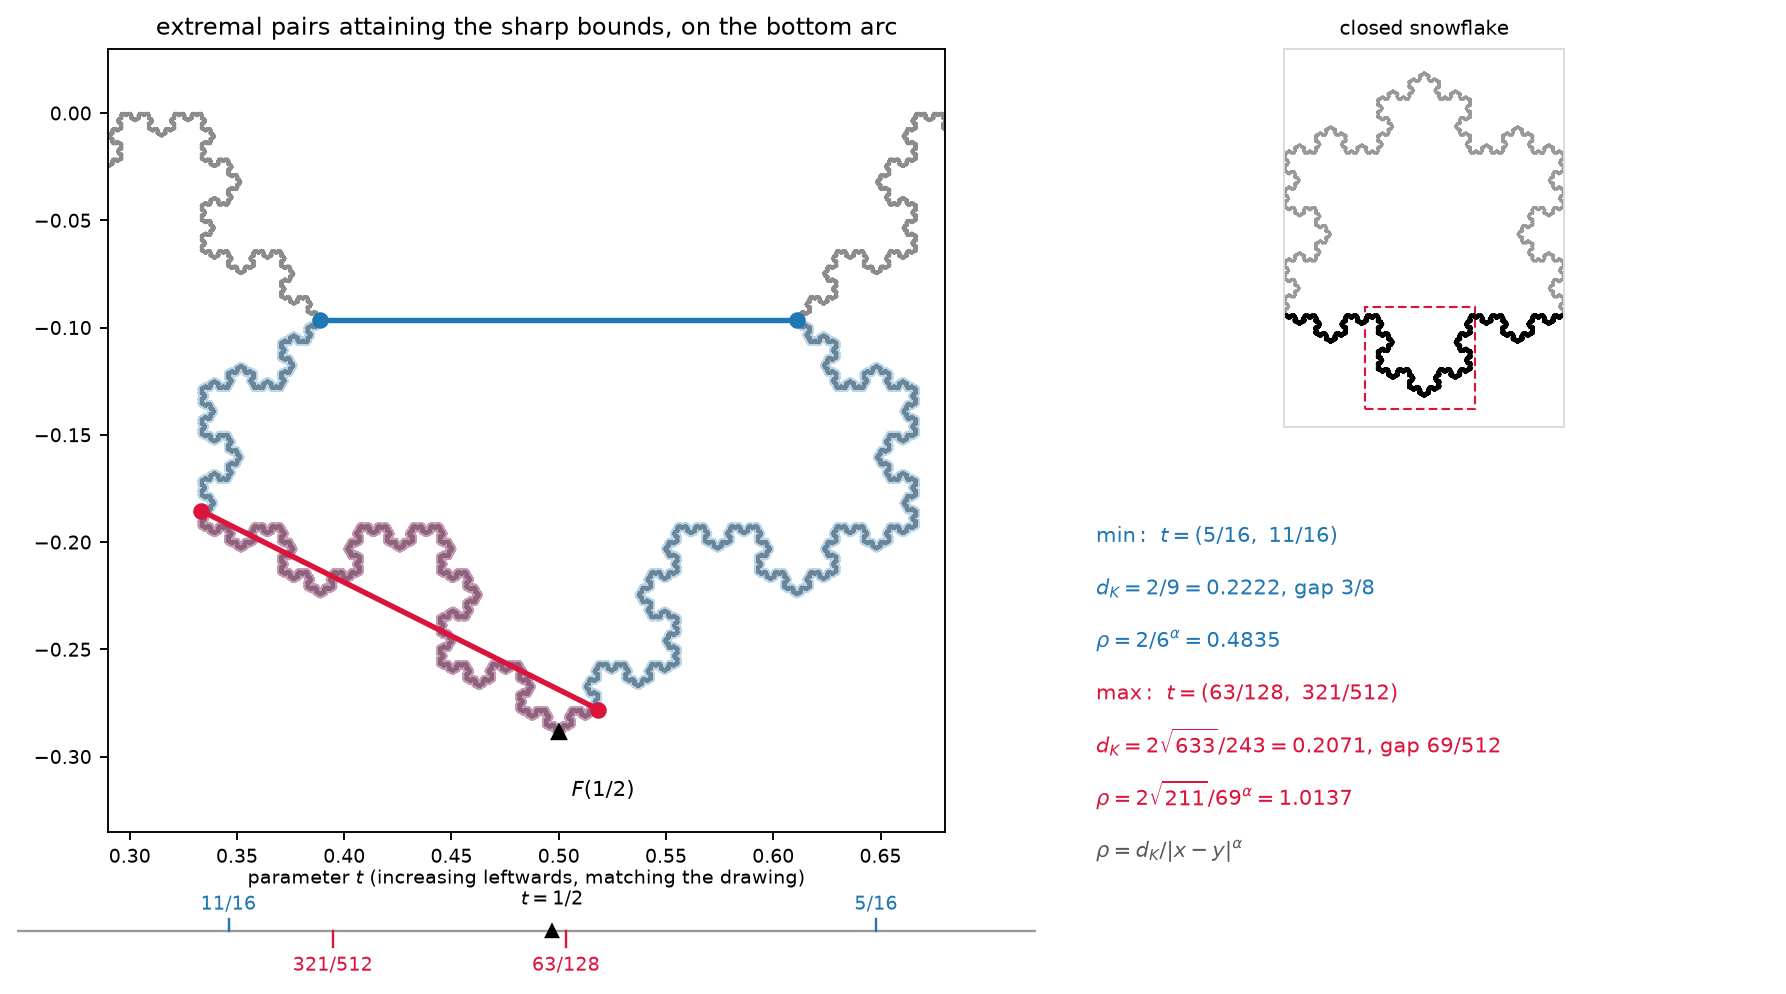
\includegraphics[width=0.74\textwidth]{koch-extremal-configurations.png}
\caption{The minimal configuration and a maximum configuration, with the flat chord $2/9$ over the
parameter gap $3/8$. The maximum is displayed using its trimmed representative; the other maximum
orbits are covered by the formulas above.}
\end{figure}

The simple checks $\rho(0,1)=\rho(0,1/4)=\rho(0,1/2)=\rho(1/4,1/2)=1$ and
$\rho(1/4,3/4)=1/\sqrt3$ are useful against the same code. The ratio of the two optimal constants
is $\sqrt{633}\,23^{-\alpha}=2.096805160875\ldots$.

\section{Two lattice facts used in the proof}
A two-generator form of $K$ is
\[
  \phi_1(z)=\frac{e^{i\pi/6}}{\sqrt3}\bar z,\qquad \phi_2(z)=1-\frac{e^{-i\pi/6}}{\sqrt3}z,
\]
with $F(t/2)=\phi_1(F(t))$ and $F(1-t/2)=\phi_2(F(t))$. Both ratios equal
$2^{-\alpha}=3^{-1/2}$. This is why the exponent is $\log_4 3$ and why binary-prefix reduction is
also exact.

The prime $\lambda=1+\w$ over the ramified rational prime $3$ is useful for keeping track of all
denominators. We have $N(\lambda)=3$, $\lambda^2=3\w$, $3=-\w^2\lambda^2$, so
$\Z[\w]=\Z[\lambda]$. The dyadic grid satisfies $\lambda^kF(M/2^k)\in\Z[\w]$, without a rounding
of $k/2$ to $\lceil k/2\rceil$ except when one insists on clearing an ordinary power of $3$:
the exponent half-power of $3$ is a genuine integral power of $\lambda$. In particular,
$F(2^{-k})=\w^{\lceil k/2\rceil}\lambda^{-k}$.

\section{Certification and reproducibility}\label{sec:repro}
The two-sided statement above is a computer-assisted theorem, not a quotation from the literature:
the extreme case had to be computed. The finite enclosure steps use exact Eisenstein arithmetic;
only $x^{\alpha}$, logarithms, and exponentials are transcendental, and these are enclosed using
directed interval arithmetic. Positive and negative controls with wrong-side targets detect the
expected extremal cells, not off-by-one errors in the partition. The minimum family and maximum
families are independently verified by exact integer arithmetic at each of their grid points.

For reproduction, see:
\begin{itemize}\small
\item \texttt{.ultramath/smwf70lym/m4/report.md}: lower-bound enclosure, family computations, and
  the sharp threshold runs ($513$ boxes with no residual at gap $\ge1/2$, $1732$ boxes at gap
  $\ge1/4$, $5477$ boxes at gap $\ge1/8$).
\item \texttt{.ultramath/smwf70lym/m7/max/report\_max.md} and \texttt{final2.py}: the complete
  maximum computation, including the sign-and-rate enclosure and output.
\item \texttt{.ultramath/smwf70lym/m7/max/output\_max.txt}: output of the maximum certificate.
\item \texttt{.ultramath/smwf70lym/m1/report.md} and \texttt{.scratch/cells.py}: the independent
  signed minimum-local certificates (used as a check, not as a substitute for directed intervals
  everywhere).
\end{itemize}
The historical grid-search evidence alone does not prove the global extrema; it selects the small
integer configurations which the subsequent exact computation certifies. The splitting of the
result into the exact reduction and two local interval proofs is what makes a subsequent
proof-assistant formalisation feasible.

The endpoint value $2\cdot6^{-\alpha}$ at $(5/16,11/16)$ has been formalised in
\texttt{lean/KochSnowflake.lean}. It defines the four self-similar maps and the coding recursion on
grid points, proves the chord $-2/9$, proves $4^{\alpha}=3$ and $2^{\alpha}=\sqrt3$, and concludes
\texttt{KochSnowflake.rho\_value\_at\_minimiser}. The file compiles with Lean 4.35/Mathlib and
contains no \texttt{sorry}, \texttt{admit} or custom axioms. Its scope is this endpoint value only:
the global lower-bound enumeration and its interval enclosures are not yet formalised.

For the literature on the snowflake metric itself (as distinct from the constants proved here), see
P.~Assouad, \emph{Plongements lipschitziens dans $\R^n$}, Bull.\ SMF \textbf{111} (1983);
J.~Heinonen, \emph{Lectures on Lipschitz Analysis}, Jyväskylä Report 100 (2005), Remark 2.15;
J.~T.~Tyson and J.-M.~Wu, \emph{Characterisations of snowflake metric spaces},
Ann.\ Acad.\ Sci.\ Fenn.\ Math.\ \textbf{30} (2005). These sources record the exponent and the
characterisation of snowflake metric spaces, not these two optimal bi-Lipschitz constants. I have
not found these constants recorded in published form; that negative literature claim is not part
of the proof.

\end{document}
